\documentclass[12pt]{report}
 
\usepackage[latin1]{inputenc}
\usepackage[T1]{fontenc}
\usepackage[francais]{babel}
 
\usepackage{graphicx}
\begin{document}
 
\begin{table}
\begin{center}
\begin{tabular}{|c|c|}
\hline
1 & 2 \\
\hline
3 & 4 \\
\hline
\end{tabular}
\end{center}
\caption[Un tableau]{Mon beau tableau}
\end{table}
 
\begin{figure}
\begin{center}
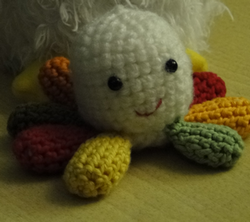
\includegraphics{poulpy.png} 
\end{center}
\caption{Poulpy est multicolore}
\end{figure}
 
\begin{figure}
\begin{center}
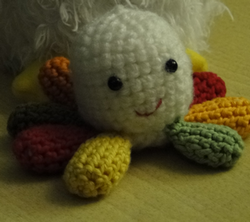
\includegraphics{poulpy.png} 
\end{center}
\caption[Chatoyante]{Poulpy est chatoyante}
\end{figure}
 
\begin{figure}
\begin{center}
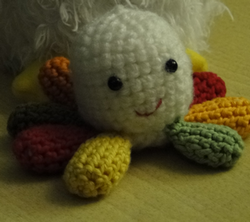
\includegraphics{poulpy.png} 
\end{center}
\caption{Poulpy est inestimable}
\end{figure}
 
\begin{table}
\begin{center}
\begin{tabular}{|c|c|}
\hline
1 & 2 \\
\hline
3 & 4 \\
\hline
\end{tabular}
\end{center}
\caption{Mon beau tableau}
\end{table}
 
\begin{figure}
\begin{center}
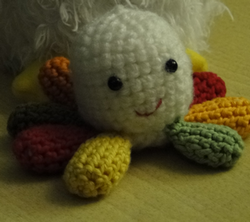
\includegraphics{poulpy.png} 
\end{center}
\caption[Poulpesque]{Poulpy est poulpesque}
  
\end{figure}
 
\listoftables
\listoffigures
 
\end{document}